\documentclass[tikz,border=10pt]{standalone}
\usetikzlibrary{calc}
% Scale s = 0.013201 cm/px, origin at A, y flipped
\begin{document}
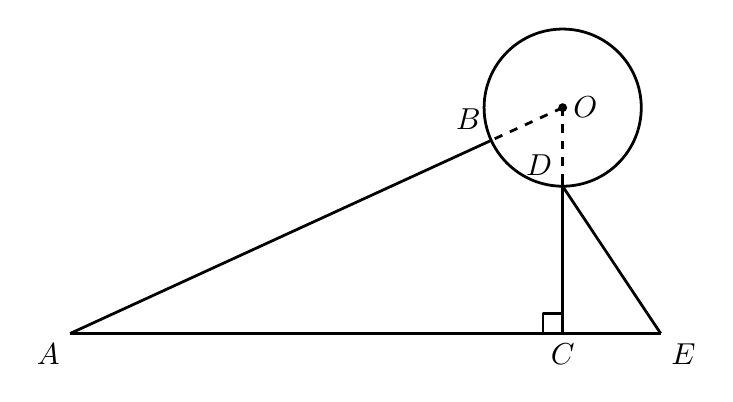
\begin{tikzpicture}[line width=1.0pt, line join=round]
  % Named coordinates (cm)
  \coordinate (A) at (0,0);
  \coordinate (E) at (7.499,0);
  \coordinate (C) at (6.254,0);
  \coordinate (U) at (6.003,0);   % right-angle mark corner
  \coordinate (D) at (6.254,1.868);
  \coordinate (O) at (6.254,2.868);
  \coordinate (B) at (5.346,2.452);
  \coordinate (Dtop) at (6.254,2.007); % CD overhang ~10 px above D

  % Full circle, radius 0.998 cm
  \draw (O) circle (0.998);

  % Baseline A–E
  \draw (A) -- (E);
  % A–B stops at B
  \draw (A) -- (B);
  % D–E
  \draw (E) -- (D);
  % Vertical C–Dtop (keeps the >=10 px overhang above D)
  \draw (C) -- (Dtop);

  % Dashed radii O–B and O–D
  \draw[dashed] (O) -- (B);
  \draw[dashed] (O) -- (D);

  % Right-angle mark at C (side 19 px = 0.251 cm), one mark only
  \draw (U) -- ($(U)+(0,0.251)$) -- ($(C)+(0,0.251)$);

  % Centre dot
  \fill (O) circle (1.6pt);

  % Labels
  \node[below left, font=\fontsize{10.5}{12.6}\selectfont] at (A) {$A$};
  \node[above left, font=\fontsize{10.5}{12.6}\selectfont] at (B) {$B$};
  \node[right, font=\fontsize{10.5}{12.6}\selectfont] at (O) {$O$};
  \node[above left, font=\fontsize{10.5}{12.6}\selectfont] at (D) {$D$};
  \node[below, font=\fontsize{10.5}{12.6}\selectfont] at (C) {$C$};
  \node[below right, font=\fontsize{10.5}{12.6}\selectfont] at (E) {$E$};
\end{tikzpicture}
\end{document}